

\subsubsection{Formali semantika}

\subsubsection{Semantinės domeno sritys}

Abstraktkti laiko domeno sritis yra vadinama \textit{Time}. Abstrakti polimorfinio elgesio(\textit{$\alpha$-behaviors}) domeno sritis yra žymima \textit{Behavior_{\(\alpha\)}}, o polimorfinių įvykių(\textit{$\alpha$-events}) yra žymima \textit{Event_{\(\alpha\)}}.

Daugiausia šių sričių (sveikieji skaičiai, loginės reikšmės) yra standartinės ir nereikalauja paaiškinimo. \textit{Time} domeno sritis reikalauja specialaus traktavimo kadangi laiko reikšmės įtraukia dalinius elementus. Ypač yra žinoma, jog laikas bent jau kažkokia reikšmė netgi nežinant galutinės reikšmės. Tiksliau laiko domeno sritį galima apibrėžti taip: tarkime \textit{R} yra rinkinys realių skaičių ir jame yra elementai \(\infty\)  ir -\(\infty\). Šis rinkinys turi standartinį aritmenį rikiavimą \(\leq\) įskaitant faktą, jog -\(\infty\) \(\leq\) \(\infty\) kiekvienam x \(\in\) R.

Dabar apibrėžkime laiką kaip \textit{Time} = R + R, kur elementai antrame rinkinyje R yra atskiriami rikiaviu \(\geq\) (pavyzdžiui, \(\geq\) 42 skaitytume kaip "daugiau arba lygu 42". Tada galima apibrėžti \perp \textit{Time} =  \(\geq\)(-\(\infty\)) ir domeno srities (pavyzdžiui, informacijos) rikiavimą pagal laiką:

\begin{gather*}
x \(\sqsubseteq\) x, \(\forall\)x \in R \\
\(\geq\)x \(\sqsubseteq\) y  if x \(\leq\) y, \(\forall\)x,y \in R \\
\(\geq\)x \(\sqsubseteq\) \(\geq\) y if x \(\leq\) y, \(\forall\)x,y \in R
\end{gather*} 

Lengva pastebėti, jog \(\perp\)\textit{Time} yra apatinis elementas. Svarbu paminėti, jog y yra tik bent viršutinė dalinių elementų rinkinio riba (angl. leat upper bound), kuri apytiksliai lygi:

\begin{gather*}
y = \sqcup\ \{ \geq\ \(\|\) x \leq\ y \}
\end{gather*} 

Kadangi laiko domeno rikiavimas yra grandinės tipo ir kiekviena tokia grandinė turi bent viršutinę ribą (prisiminkime R turi viršutinį elementą \(\infty\)), laiko domenas yra pilnos dalinės tvarkos (angl. complete partial order). Šis faktas yra būtinas, jog būtų galima užtikrinti, kad rekursyvūs apibrėžimai yra gerai apibrėžti.

\textit{Time} rinkinio elementai naudingiausi įvertinant laiką kada atsitinka įvykis. Įvykis kurio laikas apytiksliai \(\geq\)t yra tas, kurio konkretus įvykimo laikas yra didesnis nei t. Svarbu, jog įvykio, kuris niekada neįvyksta, laikas yra \(\infty\), bent viršutinė R riba.

Galiausiai apibrėžimą galima išplėsti aritmetiniui operatoriui \(\leq\) visam \textit{Time} apibrėžiant jo elgesį visuose subdomenuose:

\begin{gather*}
x \(\leq\) _\(\geq\)y if x \leq y
\end{gather*}

Tai gali būti skaitoma kaip: "Laikas x yra mažesnis arba lygus laikui, kuris yra bent y jeigu x mažiau arba lygu y". Lengva parodyti, jog ši išplėsta tipo \texit{Time} \(\rightarrow\) \textit{Time} \(\rightarrow\) \textit{Bool} funkcija yra tolydi atsižvelgiant į \(\sqsubseteq\).

\subsubsection{Semantinės funkcijos}

Polimornio elgesio interpretaciją galima apibrėžti kaip funkciją, kuri priima polimorfinę reikšmę bei pagamina elgesio b reikšmę  laiku t.

\begin{gather*}
at : Behavior_{\alpha} \(\rightarrow\) Time \(\rightarrow\) \alpha
\end{gather*}

Tada galima apibrėžti polimorfinių įvykių interpretaciją kaip paprastą ir negriežtą \textit{Time} \(\times\) \(\alpha\) porą, aprašančią laiką ir informaciją, susijusią su įvykio atsitikimu:

\begin{gather*}
occ : Event{\alpha} \(\rightarrow\) Time \(\times\) \alpha
\end{gather*}

Žinant semantinę domeno sritį, galima pateikti formalias įvykių kombinatorių interpretacijas.

\subsubsection{Elgesio semantika}

Elgesys yra kuriamas iš kito elgesio, statinių (nesikeičiančių laike) reikšmių ir įvykių naudojantis kolekcija konstruktorių (kombinatorių).

\begin{itemize}
	
	\item \textbf{Laikas}. Paprasčiausias primityvus elgesys yra laikas - \text{time}, kurio semantika yra:

\begin{gather*}
time: Behavior_{Time} \\
\textbf{at}[[time]]t = t
\end{gather*}

	Šiuo atveju \textbf{at}[[time]]t = t yra tik \textit{Time} tapatumo funkcija.

	\item \textbf{Pakėlimas\footnote{Praktikoje pakėlimas yra reikalingas gana dažnai, todėl būtų nepatogu visur kelti išreikštinai. Vietoje to pageidautina naudoti žinomus vardus, tokius kaip: "sin", "cos", "+", "*"\ ir netgi literalus, tokius kaip "3"\ arba "mėlynas"\ nurodant pakeltas versijas. Pavyzdžiui, literalas "42"\ turėtų elgtis kaip nekintantis elgesys "\(lift_{0}\) 42", o sudėtis "b_{1}\ + b_{2}"\ - "\(lift_{2}\) (+)\ \(b_{1}\) \(b_{2})"}} (angl. lifting) - įprastas būdas funkcijoms, apibrėžiančioms nekintančias reikšmes, "pakelti" į analogines funkcijas, apibrėžtoms elgesiu. Pakėlimas yra įvykdomas naudojant (konceptualiai begalinę) šeimą operatorių - vieną keikvienam funkcijos valentingumui (angl. arity).

\begin{gather*}
lift_{n} : ( \alpha_{1} \rightarrow\ ... \rightarrow\ \alpha_{n} \rightarrow\ \beta ) \rightarrow\
	Behavior_{\alpha_{1}} \rightarrow\ ... \rightarrow\ Behavior_{\alpha_{n}} \rightarrow\ Behavior_{\beta} \\
\textbf{at}[[lift_{n} f b_{1}...b_{n}]]t = f (\textbf{at}[[b_{1}t]])...(\textbf{at}[[b_{n}]]t)
\end{gather*}

	Svarbu paminėti, jog nesikeičiančios reikšmės pakėlimas yra \textit{lift_{0}}

	\item \textbf{Laiko transformacija}. Laiko transformacija leidžia vartotojui pakeisti lokalų laikotarpį. Toks būdas palaiko bet kokio elgesio laikiną modalumą. (Panašiai 2D ir 3D transformacijos palaiko erdvinį modalumą geometrijoje)

\begin{gather*}
timetransform : Behavior_{\alpha} \rightarrow\ Behavior_{Time} \rightarrow\ Behavior_{\alpha} \\
\textbf{at}[[timeTransform b tb]] = \textbf{at}[[b]] o \textbf{at}[[tb]]
\end{gather*}

Taigi idėja yra, jog laikas yra \textit{timeTransform} tapatybė:

\begin{gather*}
timeTransform\ b\ time = b
\end{gather*}

Pavyzdžiui, laiko transformacijos pavyzdys Fran:

\begin{gather*}
timeTransform\ b\ (time/2)
\end{gather*}

sulėtina animaciją dvigubai.

	\item \textbf{Integracija}. Integracija pritaikoma tiek realių skaičių reikšmes turinčiam, tiek 2D ir 3D vektoriaus reikšmes turinčiam elgesiui, arba apskritai vektoriaus erdvei (limituota). Naudojant Haskell notaciją vektoriaus erdvei:

\begin{gather*}
integral: VectorSpace\ \(\alpha\) \Rightarrow\ Behavior_{\alpha} \rightarrow\ Time \rightarrow\ Behavior_{\alpha} \\ 
\textbf{at}[[integral b t_{0}]]t = [ \int_\(t_{0}\)^t \textbf{at}[[b]]]
\end{gather*}

	Integracija leidžia specifikuoti elgesio greitį, o naudojama du kartus pagreitį. Pavyzdžiui, judančio kamuoliuko greitis yra duotas kaip elgesys b (gali būti ir pastovus ir nepastovus), tada jo reliatyvi pozicija laiko pradžios atžvilgiu \(t_{0}\)\ yra duota kaip \textit{integral b \(t_{0}\)}. Tai leidžia natūraliai išreikšti fizika paremtas animacijas.

	\item \textbf{Reaktyvumas}. Pagrindinė sąveika yra tarp elgesio ir įvykių ir tai padaro elgesį reaktyviu. Konkrečiai elgesys \textit{b untilB e} parodo b elgesį iki tol kol įvyksta e ir tada pasikeičia į elgesį asocijuotą su įvykiu e. Formaliai:

\begin{gather*}
untilB : Behavior_{\alpha} \rightarrow\ Event_{Behavior_{\(\alpha)}} \rightarrow\ Behavior_{\alpha} \\
\textbf{at}[[b\ untilB\ e]]t = if\ t \leq t_{e} \textbf{ then at}[[b]]t\ \textbf{else at}[[b']]t \\
\textbf{where} (t_{e}, b') = \textbf{occ}[[e]]
\end{gather*}

\end{itemize}

\subsubsection{Įvykių semantika}

\begin{itemize}

	\item \textbf{Įvykių apdorojimas}. Norint duoti pavyzdį naudojant specialią rūšį įvykių, pirmiausia reikia apibrėžti įvykių apdorotojus, kurie yra pritaikomi laikui ir su įvykiu susietiem duomenim naudojant šį operatorių:

\begin{figure}[H]
	\centering
	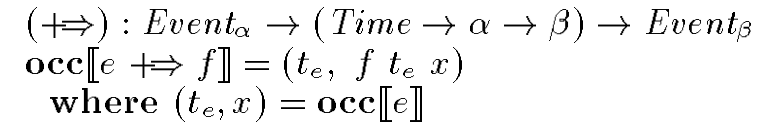
\includegraphics[scale=0.75]{pics/1.png}
	\label{pic:1}
\end{figure}

	Patogumui galima naudoti šias išvestas ooperacijas, kurios ignoruoja laiką arba informaciją arba abu kartu:

\begin{figure}[H]
	\centering
	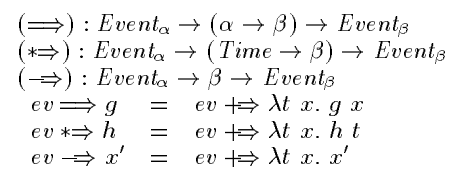
\includegraphics[scale=0.75]{pics/2.png}
	\label{pic:2}
\end{figure}

	(+$\Rightarrow$) gauna visus parametrus, (-$\Rightarrow$)  negauna parametrų, (*$\Rightarrow$) gauna tik laiką, o ($\Longrightarrow$) gauna tik informaciją.

	\item \textbf{Nekintantys įvykiai}. Paprasčiausia įvykių rūšis yra tiesiogiai specifikuoti pagal laiką ir reikšmę.

\begin{figure}[H]
	\centering
	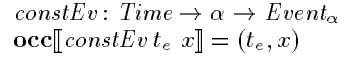
\includegraphics[scale=0.75]{pics/3.png}
	\label{pic:3}
\end{figure}

	Nors, pavyzdžiui, elgesys:

\begin{figure}[H]
	\centering
	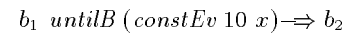
\includegraphics[scale=0.75]{pics/4.png}
	\label{pic:4}
\end{figure}

	parodo elgesį \(b_{1}\) iki laiko taško 10, kuriame jis pradeda rodyti elgesį \(b_{2}\) (x yra ignoruojamas šiame pavyzdyje, bet iš tikro neturėtų).

	\item \textbf{Išoriniai įvykiai}. Išoriniai įvykiai yra pavyzdžiui pelės mygtuko paspaudimas, kuris gali būti kairysis arba dešinysis mygtukas. Reikšmė, asocijuota su kurio nors mygtuko paspaudimu yra interpretuojama kaip atleidimo įvykis, kuris grąžina vienetinę reikšmę (() yra vieneto tipas):

\begin{figure}[H]
	\centering
	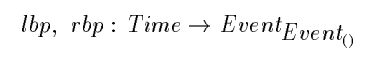
\includegraphics[scale=0.75]{pics/5.png}
	\label{pic:5}
\end{figure}

	Įvykio \textit{lbp \(t_{0}\)} prasmė, pavyzdžiui, yra pora (\(t_{e}\), e), tokia kad \(t_{e}\) yra pirmojo kairio mygtuko paspaudimas po laiko \(t_{0}\) ir \textit{e} yra įvykis, reiškiantis pirmojo kairiojo mygtuko atleidimą po laiko \(t_{e}\). Iš to seka, jog:

\begin{figure}[H]
	\centering
	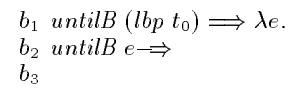
\includegraphics[scale=0.75]{pics/6.png}
	\label{pic:6}
\end{figure}

	parodo elgesį \(b_{1}\) iki kairiojo mygtuko paspaudimo, kurio metu jis tampa \(b_{2}\) kol kairysis mygtukas yra atleistas, o tada tampa \(t_{3}\).

	\item \textbf{Predikatai}. Natūralus būdas specifikuoti tam tikrus įvykius kaip pirmąjį laiką kada loginės reikšmės elgesys tampa tiesa (\textit{true}) po duoto laiko:

\begin{figure}[H]
	\centering
	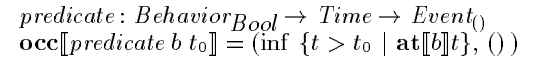
\includegraphics[scale=0.75]{pics/7.png}
	\label{pic:7}
\end{figure}

	Predikato įvykio laikas yra begalinis ir sudarytas iš rinkinio laiko taškų didesnių tei \(t_{0}\), kuriuose elgesys yra teigiamas. Šis laikas gali būti ir \(t_{0}\).

	Tada elgesys:

\begin{figure}[H]
	\centering
	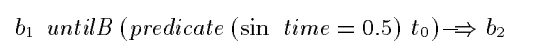
\includegraphics[scale=0.75]{pics/8.png}
	\label{pic:8}
\end{figure}

 	parodo \(b_{1}\) iki pirmojo laiko taško t po \(t_{0}\), kur \textit{sin t} yra 0.5, po kurio jis parodo \(b_{2}\).

 	\item \textbf{Pasirinkimas}. Galima pasirinkti ankstesnįjį iš dviejų įvykių naudojantis operatoriumi .|.:

\begin{figure}[H]
	\centering
	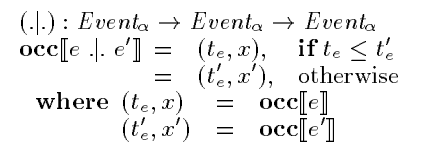
\includegraphics[scale=0.75]{pics/9.png}
	\label{pic:9}
\end{figure}

	Pavyzdžiui, elgesys:

\begin{figure}[H]
	\centering
	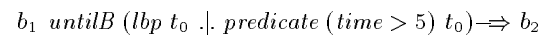
\includegraphics[scale=0.75]{pics/10.png}
	\label{pic:10}
\end{figure}

	laukia kol arba bus nuspaustas kairysis mygukas arba praeis 5 sekundės prieš pakeičiant \(b_{1}\) elgesį į \(b_{2}\). Kaip alternatyva, sekantis pavyzdys pakeičia elgesį į \(b_{3}\) po skirto laiko pabaigos:

\begin{figure}[H]
	\centering
	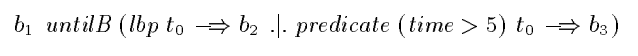
\includegraphics[scale=0.75]{pics/11.png}
	\label{pic:11}
\end{figure}

	\item \textbf{Momentinė kopija}. Tuo momentu kai nutinka įvykis yra dažnai patogu padaryti elgesio reikšmės momentinę kopiją tam tikrame laiko taške. Tai formaliai galima užrašyti:

\begin{figure}[H]
	\centering
	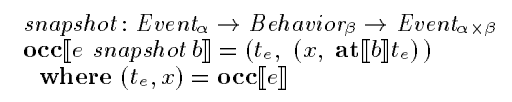
\includegraphics[scale=0.75]{pics/12.png}
	\label{pic:12}
\end{figure}

	Pavyzdžiui, elgesys:

\begin{figure}[H]
	\centering
	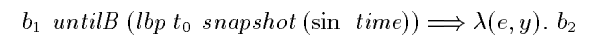
\includegraphics[scale=0.75]{pics/13.png}
	\label{pic:13}
\end{figure}

	paima laiko, kai yra nuspaudžiamas kairysis mygtukas, sinusą, priskiria jį \textit{y} ir seka elgesiu \(b_{2}\), kuris galimai priklauso nuo \textit{y}. Nepaisant to, šį pavyzdį taip pat būtų galima realizuoti paimant kairiojo mygtuko paspaudimo įvykio laiką ir skaičiuojant sinusą, bendru atveju elgesio buvimas momentine kopija yra ganėtinai sudėtingas ir gali priklausyti nuo išorinių įvykių.

	\item \textbf{Įvykių sekos} Kartais yra naudinga naudoti vieną įvykį, kad būtų galima sukurti kitą. Įvykis \textit{joinEv e} yra įvykio, kuris nutinka kai nutinka \textit{e'}, kur \textit{e'} yra \textit{e} reikšmės dalis:

\begin{figure}[H]
	\centering
	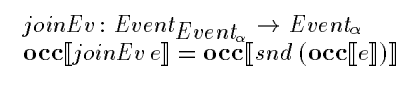
\includegraphics[scale=0.75]{pics/14.png}
	\label{pic:14}
\end{figure}

	Pavyzdžiui, įvykis:

\begin{figure}[H]
	\centering
	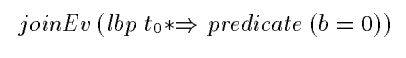
\includegraphics[scale=0.75]{pics/15.png}
	\label{pic:15}
\end{figure}

	nutinka pirmą kartą kai elgesys \textit{b} turi nulinę reikšmę po pirmojo kairiojo mygtuko paspaudimo po laiko tarpo \(t_{0}\).

\end{itemize}

\subsubsection{Panaudojimo pavyzdys}

Praeitas skyrius pateikė primityvių kombinatorių pavyzdžius elgesiui bei įvykiam kartu su jų formalia semantika. Remiantis šia semantika pateiksime pavyzdį dalį šių kombinatorių Haskell programavimo kalboje. \ref{sign} pateiktame pavyzdyje yra skaitine reikšme išreikštas elgesys, kurio pradinė reikšmė yra 0 ir tampa -1 jeigu yra nuspaustas kairys pelės mygtukas arba 1 jeigu yra nuspaustas dešinys pelės mygtukas.

\begin{lstlisting}[caption=- signalo funkcija nuo pelės mygtuko paspaudimo, label=sign]
	bSign t0 =
		0 'untilB' lbp t0 ==> nonZero (-1) .|.
				   rbp t0 ==> nonZero 1
		where nonZero r stop =
				r 'untilB' stop *=> bSign
\end{lstlisting}

Šį elgesį galima panaudoti paveikslėlio dydžio keitimui. Kairio arba dešinio pelės mygtuko paspaudimas priverčia paveikslėlį padidėti arba sumažėti. Pavyzdys pateiktas \ref{grow}.


\begin{lstlisting}[caption=- paveiksliuko dydžio modifikavimas pelės paspaudimu, label=grow]
	bSign t0 =
		0 'untilB' lbp t0 ==> nonZero (-1) .|.
				   rbp t0 ==> nonZero 1
		where nonZero r stop =
				r 'untilB' stop *=> bSign
\end{lstlisting}





